
\textit{Randomized benchmarking}~\cite{Magesan2012, Kelly2014, Proctor2019, Chow2009} (RB) is the collective name of a series of popular protocols for characterizing the quality of a quantum processor.
In particular, the objective of RB is to give a single value that describes the fidelity of a general gate.
Here we talk about \textit{gate fidelity} that is a parameter much more important than the \textit{assignment fidelity} that we encountered in the last experiments.

Different RB protocols currently exist and are used, but they all share one core idea.
They consist in the generation of random Clifford circuits plus their conjugates, so that the application of both should be equal to the identity.
We repeat the experiment for increasing depths of the circuits and we extract the error rate per single qubit from the resulting exponential decay.

With Clifford circuit we intend a circuit composed of gates from the universal Clifford set.

\subsection*{Standard Randomized Benchmarking}

With the standard version of the experiment we can compute an average gate fidelity or a fidelity differentiated between the different Cliffords.\\
The experiment is conceptually simple:
\begin{itemize}
    \item we choose a maximum, a minimum and a step depth for the scan;
    \item for a given depth, we randomly generate a circuit;
    \item we execute the circuit $C$ applying $C^\dagger C \ket 0$;
    \item we measure and iterate for all the chosen depths.
\end{itemize}

A usual plot for the standard RB is presented in \cref{fig:sketch_rb}.
\begin{figure}[ht]
    \centering
    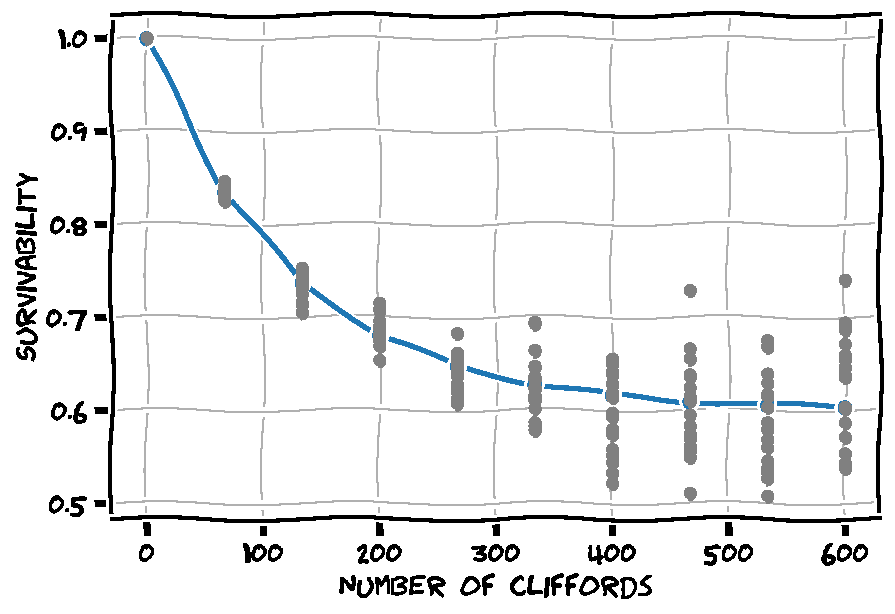
\includegraphics[width=8cm]{characterization/figures/rb_sketch.pdf}
    \caption{Sketch of the plot of a standard randomized benchmarking experiment .}
    \label{fig:sketch_rb}
\end{figure}

We can easily compute the averaged error per gate $\mathcal E=1-\epsilon$ ($\epsilon$ is the fidelity) by fitting the curve with:
\begin{equation}
    y = A\epsilon^{n} + B
\end{equation}
where $n$ is the number of gates for circuit.

To compute the error related to a specific gate $e_i$ we can use:
\begin{equation}
    \mathcal E = 1 - \prod_i(1-e_i)^n_i \sim \sum_i n_i e_i + O(e^2)
\end{equation}
It seems that we cannot distinguish the values of $\mathcal E$ and $e_i$, however by defining an error ratio $r_i$, with respect to a chosen value $e_0$ we can compute the error for each basis gate:
\begin{equation}
    \mathcal E \sim e_0 \sum_i n_i r_i \rightarrow e_i \sim r_i e_0 = \frac{r_i \mathcal E}{\sum_i n_i r_i}
\end{equation}

The \textit{pulse fidelity}, often used as figure of merit for qubit characterization, has a definition derived from the fidelity:
\begin{equation}
    \text{pulse fidelity} = 1-\frac{\frac{1-\epsilon}{2}}{\text{num pulses per Clifford}\approx1.85}
\end{equation}

In general, this experiment can be complex to perform with success on hardware: in particular if you are trying to reach high fidelities (we usually "count the 9s": 0.98, 0.998, 0.9998...) it usually involves very long sequences (since at lower depths the curve should be almost flat).
In particular for the \RFSoC it proved to be a problem, since the long sequences (for 3 nines 500 gates are needed) filled the limited memory available.
For example, the experiment presented in \cref{fig:rb_short} would be much more reliable if it did reach depths of 100/200.

\begin{figure}[ht]
    \centering
    \makebox[\textwidth][c]{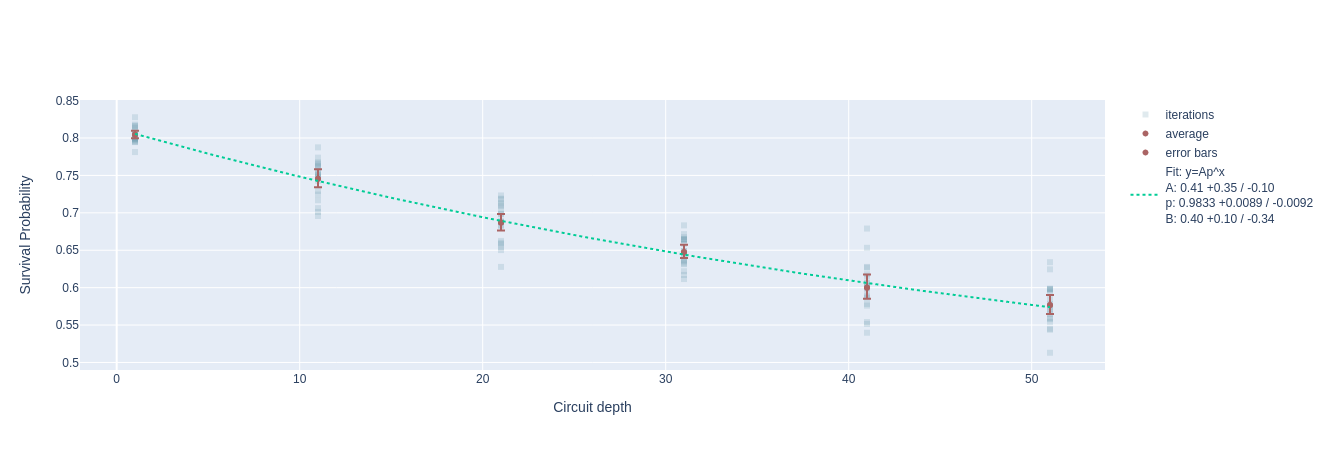
\includegraphics[width=1.3\textwidth]{characterization/figures/rb_short.png}}
    \caption{Plot of a standard randomized benchmarking experiment executed with a \RFSoC.}
    \label{fig:rb_short}
\end{figure}

Note that in this experiment is advised to not use a large number of shots, but rather to execute multiple time the circuit with different Cliffords, hence the different iterations present in the plots.


